\graphicspath{{./figures/}}

\section{Problem Statement}

The initial problem statement provided was simply to design a communication system for a PocketQube, with focus on the ground station. As this statement is relatively broad, further investigation is necessary to clearly defined the problem. The requirements for this project are therefore defined by analysing general, currently existing balloon-satellite systems, as well as taking into account the planned launch that this specific PocketQube is planned to be used in, as shown in Figure \ref{fig:balloon_path}. Further, the existing radiosonde (an iMet-54 atmospheric telemetry device) is used as a reference, both for the new system's requirements, and as a consideration for system integration.

\begin{figure}[!htb]
  \centering
  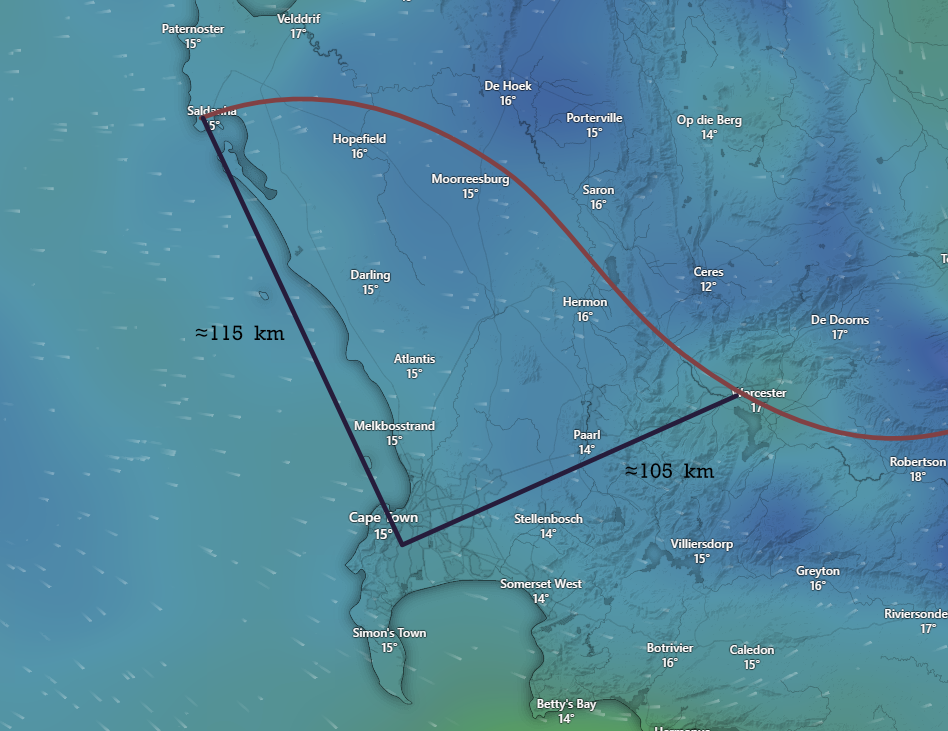
\includegraphics[width=0.6\textwidth]{balloon_path}
  \caption{Planned Balloon Path and Distances}
  \label{fig:balloon_path}
\end{figure}

Generally, high-altitude balloons can drift to a height as much as 30 km above sea level \cite{site-weatherWeatherBalloons}. For this project, the balloon is planned to be released from near Saldanha Bay, where it could travel a maximum distance of around 200 km towards the Cederberg, and land furthest in Worcester. From Cape Town, this is a maximum straight line distance of around 115 km. 

A ground station should maintain a reliable wireless link with a satellite to enable continuous communication. real-time data transmission and telemetry should be maintained. Since most radiosondes are simply uni-directional "downlink" devices, this should be a priority requirement, however ground stations sometimes are also capable of simple bi-directional communication.